\section{Aritmetica dei calcolatori}

\subsection{Somma e Sottrazione}
Per eseguire l'addizione di due numeri in complemento 
a due dobbiamo eseguire l'addizione bit a bit considerando il riporto.
Mentre per eseguire la sottrazione dobbiamo prima eseguire il complemetno 
a due del secondo membro e poi eseguire la somma.
\paragraph{Overflow}
L'overflow può avvenire quando si esegue la somma di due 
numeri con lo stesso segno oppure quando di esegue la sottrazione di 
numeri con segno opposto.Per identificare l'overflow dobbiamo vedere il 
bit del segno, dato che se i bit del valore non bastano a rappresentare il numero
allora il bit del segno verrà impostato a 1 nel caso di positivi e 0 nel caso di negativi.

\paragraph{Overlflow negli unsigned}
Nei valori unsigned per verificare l'overflow nella somma,
dobbiamo controllare che il risultato sia maggiore dei due
operandi, in caso contrario c'è stato un overflow.
Mentre nella sottrazione dobbiamo verificare che il 
risultato sia minore del minuendo.In caso contrario c'è stato un overflow.
\subsection{Moltiplicazione}

L'hardware per la moltiplicazione è molto simile al modo in cui si esegue la moltiplicazione su carta.

\begin{figure}[H]
    \centering
    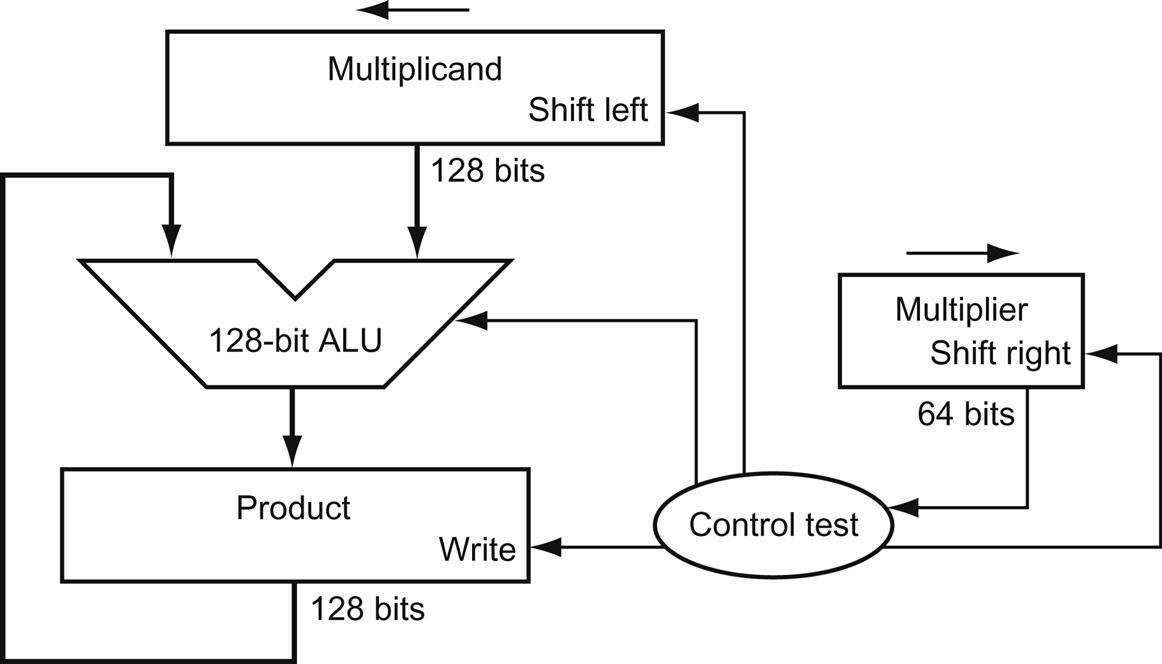
\includegraphics[width=100mm,scale=1.5]{pictures/schemaMoltiplicazione.png}
    \caption{HW moltiplicazione}
    \label{fig:hw-multiplication}
\end{figure}
\newpage
Il control test esegue per 64 volte il seguente algoritmo:
\begin{enumerate}
    \item Controlla che il bit meno valente del moltiplicatore:
    \begin{enumerate}
        \item Se il bit è a 1, allora somma il moltiplicando al prodotto.
        \item Se il bit è a 0, non fa nulla.
    \end{enumerate}
    \item Esegue lo shift left del moltiplicando e lo shift right del moltiplicatore.
\end{enumerate}
\subsubsection{Moltiplicazione più veloce}
Questo hardware può essere rifinito per essere più veloce ed economico.

\begin{figure}[H]
    \centering
    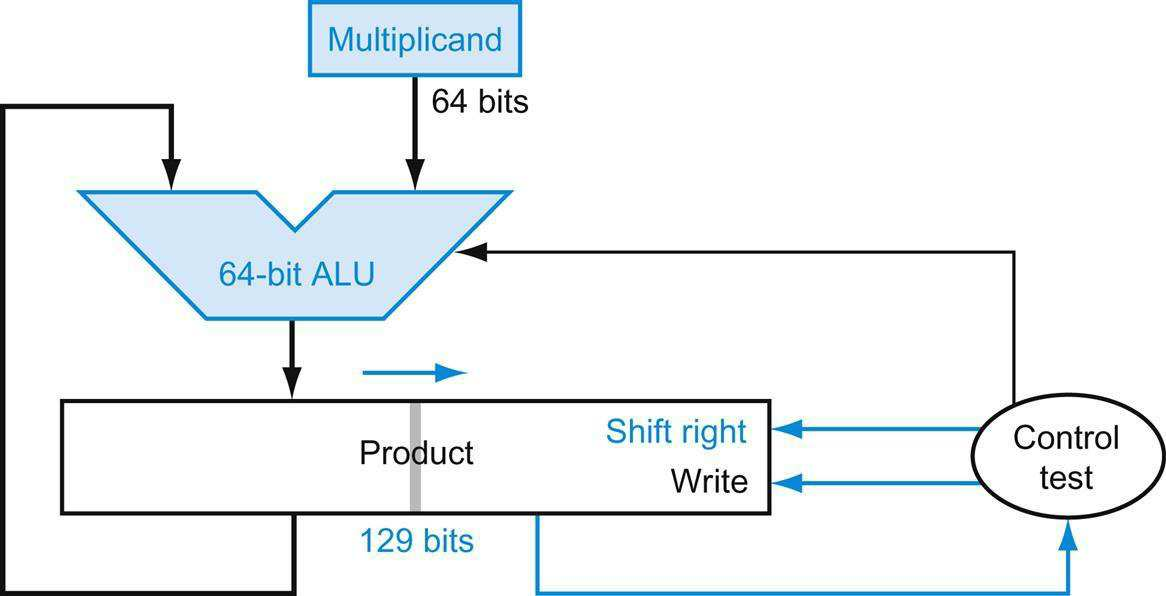
\includegraphics[width=100mm,scale=1.5]{pictures/schemaMoltiplicazioneVeloce.png}
    \caption{HW moltiplicazione veloce}
    \label{fig:hw-multiplication}
\end{figure}

L'aumento di velocità deriva dall'esecuzione in parallelo, in questo caso lo shift di moltiplicando e moltiplicatore vengono eseguiti 
mentre il moltiplicando viene sommato al prodotto. L'HW deve assicurarsi di testare il giusto bit del moltiplicatore e di 
prendere la versione shiftata del moltiplicando. È più economico perchè non ci serve più una ALU a 128 bits e risparmiamo un 
registro da 128 bits. 

\subsection{Divisione}
